\documentclass[openany]{article}
\usepackage[a4paper,margin=1in,bottom=1.5in]{geometry} % define margins. Bottom margin is used to lift a little bit the page number.
\usepackage[english]{babel} % document language is english
\usepackage[dvipsnames]{xcolor} % used for creating colored boxes
\usepackage{graphicx} % for including images
\usepackage[export]{adjustbox}
\usepackage{fancyhdr} % used for creating headers and footers. only used in title page in this document.
\usepackage{tabularx} % creation of more complex tables
\usepackage{array} % allow elements of tabular environment to have vertical alignment, e.g., center alignment.
\usepackage{nameref} % make it possible to reference by name
\usepackage{hyperref} % allow hiperlinks (links to other document parts and extern links)
\usepackage{etoc} % used for generation of section local table of contents
\usepackage{placeins} % allows the use of float barriers, preventing figures and tables to be placed in inconvenient places

% Define graphics path
\graphicspath{{figs/}}

% Configure the cross reference hyper links color
\hypersetup{
    colorlinks=true,
    linkcolor=blue,
}

\newcolumntype{C}{>{\centering\arraybackslash}X} % new column type for tabularx
						 % centered (\centering), adjust width in order to fill table width (X type)

% Configure header in 'titlepage'
\pagestyle{fancy}
\lhead{
\includegraphics[width=4.5cm]{logo_cnpem}}
\rhead{
\includegraphics[width=4cm]{logo_lnls}}
\renewcommand{\headrulewidth}{0pt}
\setlength{\headheight}{52pt}
% Clean footer
\fancyfoot{}

% increase table height factor a little bit (taller cells)
\renewcommand{\arraystretch}{1.5}

%==== Begin DOCUMENT ====
\begin{document}

%--- Begin title page ---
\begin{titlepage}

% Add header to this page
\thispagestyle{fancy}

% Center elements
\begin{center}

% title of title page
\topskip0pt % perfectly centered
\vspace*{\fill}
\textbf{\Huge IOC User Guide}\\[20pt]
\textbf{\Huge Version 1.0}\\[20pt]
\textbf{\Huge February/2017}
\vspace*{\fill}

% footer of title page
\vfill
\textbf{Beam Diagnostics Group (DIG)}\\[5pt]
\textbf{Brazilian Synchrotron Light Laboratory (LNLS)}\\[5pt]
\textbf{Brazilian Center for Research in Energy and Materials (CNPEM)}
\end{center}

\end{titlepage}
%--- End of title page ---

\newpage
\pagestyle{plain} % restore default page style

%--- About this manual ---
\paragraph{}{\Large\bfseries About this manual}

\paragraph{} This guide provides information and instructions about the setup and operation of the Timing System IOC. Information about the timing system hardware, or firmware can be found in the corresponding manuals.

%--- Table of contents ---
\tableofcontents

\newpage
%--- Section: Overview ---
\section{Overview}

	\paragraph{} The Timing System IOC is responsible for managing and providing process variables (PVs) for control of the Timing System modules. The Timing System functions are divided into categories and presented along with the process variables needed for configuration in section \nameref{sec:system-operation}. Further detail about the PVs is presented in section \nameref{sec:process-variables}.

%--- Section: IOC Setup ---
\section{IOC Setup}

	\paragraph{} This section describes the procedure for correctly installing and configuring the IOC for use.

	\subsection{Installation}

		\paragraph{} The Timing System IOC requires EPICS base 3.14, synApps 5.8, and StreamDevice 2-7-7 installed. Make sure to provide their intallation paths to the IOC (\hyperref[sec:release-file]{RELEASE file}) before building the IOC.

	\subsection{Editing the RELEASE file}\label{sec:release-file}

		\paragraph{} The RELEASE file, located at /\textless IOC directory\textgreater/configure/RELEASE, contains the paths for external applications. Generally, this is the only file that requires modification to build the IOC in a new machine. Make sure that the paths specified in the file agree with the applications installation locations.

	\subsection{Building the IOC}

		\paragraph{} In order to build the IOC, change the working directory to the IOC top directory and run make. Clean the directory when rebuilding the IOC.

		\bigskip
		\colorbox{lightgray}{
			\begin{tabularx}{0.9\textwidth}{X}
			\emph{make clean uninstall install}
			\end{tabularx}
		}

	\subsection{Finding the modules in the network}

		\paragraph{} The Timing System modules are DHCP by default. Therefore, the next step to set up the IOC is to find each module's IP. The top directory of the Timing System IOC contains a python script for finding the Timing modules IPs called \emph{Find\_Modules.py}. The script searches for the modules using the provided subnetwork prefix.
		In order to run it, it is necessary to have python 2 installed. From the top IOC directory, the following shell command  can be used:
		
		\bigskip
		\colorbox{lightgray}{
			\begin{tabularx}{0.9\textwidth}{X}
			\emph{python Find\_Modules.py \textless network prefix\textgreater}
			\end{tabularx}
		}

		\paragraph{} The ouput is the list of connected modules. Each line shows the info for a module, that is, its type and configuration (i.e., EVO/EVG, EVO/EVR, EVO/FOUT, or EVE), followed by its IP and port. The example of figure \ref{fig:find-modules} shows the output of \emph{Find\_Modules} for a network with only an EVG module with IP 10.0.18.55, and port 50116. 

		% Find_Modules output figure
		\begin{figure}[!h]
		\caption{Find\_Modules.py output}
		\label{fig:find-modules}
		\centering
		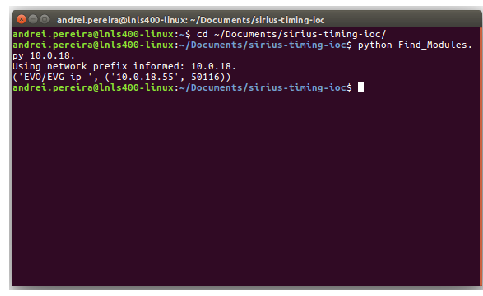
\includegraphics[width=0.8\textwidth]{find-modules-image}
		\end{figure}
\FloatBarrier

		\paragraph{} The port number is used for identifying the devices, since each Timing System module port number is unique. Table \ref{tab:port-number} presents the code and port number associated with each of the Timing System modules.
		\paragraph{} The modules' IP and port number are used for configuring the UDP/IP communication between the IOC and Timing System modules in the \hyperref[sec:startup-script]{startup script}. This procedure is described in \nameref{sec:editing-startup-script}.

		\begin{table}[!h]
		\centering
		\caption{Timing System modules Port Number}
		\label{tab:port-number}	
		\begin{tabular}{l l l}
		\bfseries Module &\bfseries Code &\bfseries Port \\ \hline
		EVO 1 & P1916001 & 50111 \\ \hline
		EVO 2 & P1916002 & 50112 \\ \hline
		EVO 3 & P1916003 & 50113 \\ \hline
		EVO 4 & P1916004 & 50114 \\ \hline
		EVO 5 & P1916005 & 50115 \\ \hline
		EVO 6 & P1916006 & 50116 \\ \hline
		EVO 7 & P1916007 & 50117 \\ \hline
		& & \\ \hline
		EVE 1 & P1816002 & 50121 \\ \hline
		EVE 2 & P1816003 & 50122 \\ \hline
		EVE 3 & P1816004 & 50123 \\ \hline
		EVE 4 & P1816005 & 50124 \\ \hline
		\end{tabular}
		\end{table}
\FloatBarrier

	\subsection{Editing the startup script}\label{sec:editing-startup-script}

		\paragraph{} The startup script should only be modified when installing the IOC in a new subnetwork, after a modification to the Timing System structure, or when a modification to the IOC initialization is desired.
		\par The script path is \emph{\textless ioc directory\textgreater /iocBoot/ioctiming/st.cmd}.

		\paragraph{} The first step when configuring the IOC in a new network is to configure the IP ports for each device that will communicate with the IOC. This is accomplished by the command \emph{drvAsynIPPortConfigure} in the startup script. For instance, suppose we have the following list of IP port configuration commands:

		\bigskip
		\colorbox{lightgray}{
			\begin{tabularx}{0.9\textwidth}{X}
			\emph{drvAsynIPPortConfigure ("EVG1", "10.0.18.55:50116:50116 udp",0,0,0)} \\
			\emph{drvAsynIPPortConfigure ("EVR1", "10.0.18.111:50111:50111 udp",0,0,0)} \\
			\emph{drvAsynIPPortConfigure ("EVR2", "10.0.18.112:50112:50112 udp",0,0,0)} \\
			\emph{drvAsynIPPortConfigure ("EVE1", "10.0.18.58:50121:50121 udp",0,0,0)} \\
			\emph{drvAsynIPPortConfigure ("EVE2", "10.0.18.54:50122:50122 udp",0,0,0)} \\
			\emph{drvAsynIPPortConfigure ("EVE3", "10.0.18.123:50123:50123 udp",0,0,0)} \\
			\end{tabularx}
		}

		\paragraph{} The first command defines a port called \emph{EVG1} with IP 10.0.18.55, port number 50116, local port number 50116, and UDP protocol.
		\paragraph{} IPs defined in the script that are no longer valid should be updated before running the IOC. IP port configuration commands can be added or commented out, depending on the number of modules used.
		\paragraph{} Further detail about configuring the IP ports is provided in section \ref{sec:ip-port-config}.

	\subsection{Running the IOC}
		% this topic should show the running procedure and expected messages in the IOC shell
		\paragraph{} In order to run the IOC, change the working directory to \emph{iocBoot/ioctiming}. Modify the \emph{st.cmd} script permission so that it can be executed:

		\bigskip
		\colorbox{lightgray}{
			\begin{tabularx}{0.9\textwidth}{X}
			chmod +x st.cmd \\
			\end{tabularx}
		}

		\paragraph{} Execute the startup script:

		\bigskip
		\colorbox{lightgray}{
			\begin{tabularx}{0.9\textwidth}{X}
			./st.cmd \\
			\end{tabularx}
		}

		\paragraph{} The IOC should start running and some messages reporting the startup status should be printed in the IOC shell. IOC misconfiguration will most likely cause error messages to be displayed during the startup procedure.

%--- Section: Timing System Operation ---
\section{Timing System Operation}\label{sec:system-operation}

	\subsection{Initialization}
		% presents what happens at IOC initialization. The automatic upload or download.
		\paragraph{} On IOC startup, the databases and sequencer programs are initialized. The autosave tool looks for save files to restore the IOC records' fields as they were in the last time that the IOC ran. The sequencer programs "EVGSetup" and "EVRESetup" check the configuration status of the timing modules. For modules that are disconfigured, a download operation is performed, transferring the select and set point parameters defined in the IOC to the module. For modules that are already configured, an upload operation is performed, transferring the module parameters to the IOC status and read-back value PVs.
		\paragraph{} The messages printed by the IOC shell are related to database, sequencer programs, and autosave initialization. Common errors and solutions are described in section \nameref{sec:common-error-causes}. 

	\subsection{Download and Upload of parameters}
		% explains the reasons or circumstances, and steps for performing a download or upload.
		\paragraph{} It is possible to download or upload parameters to/from the timing modules at any time after the IOC has initialized. This is useful when connecting the IOC to a module that is already running. If the module is configured differently from the desired and the IOC PVs contain the right settings, it is possible to tranfer the settings all at once by setting the \emph{download} PV. On the other hand, if the IOC status parameters or read-back values are not updated for some reason, setting the \emph{upload\_T} PV will update all the status and RBV PVs with the values in hardware.

	\subsection{First configuration steps}
		% guide of basic configuration and check needed for modules to operate, e.g., RFIN-Sts, ACEnbl-Sel, EVGEnbl-Sel, etc.
		\paragraph{} The first configuration steps for the timing system consist of configuring the modules inputs settings. The configuration varies from module to module, since each has its own set of inputs.

		\subsubsection{EVG}

			\paragraph{} The first step for configuring the STD-EVO as EVG is to assure that the module function has been
correctly configured by the EVG Setup sequencer program on IOC startup. The \hyperref[pvgroup:evg-configuration]{funselRBV} PV displays the module configured function. In the case that the module is incorrectly configured, it is possibble to modify the module configuration by setting the appropriate value to the \hyperref[pvgroup:evg-configuration]{funsel} PV.
			\paragraph{} As soon as the module receives a configuration, i.e., EVG, EVR, or FOUT, the \hyperref[pvgroup:evg-configuration]{alive} counter starts incrementing. Although the alive couter info may be useful, a better aproach for checking whether the device is configured is to verify the \hyperref[pvgroup:evg-module-support]{statdev} PV, which displays the device status as \emph{WAITING} when the module has not yet been configured, or \emph{RUNNING} otherwise.
			\paragraph{} The network connection status is displayed by the \hyperref[pvgroup:evg-module-support]{network} PV.
			\paragraph{} Another important step when configuring the EVG is to guarantee that both the RF clock and the \emph{event clock} are within limits. The \emph{RFIN} (RF input) must receive a signal within the range of 60 - 540MHz. The \emph{event clock} is the RF frequency divided by the \emph{RF divider}, and must be within the range of 60 - 135MHz. The \hyperref[pvgroup:evg-configuration]{rfdiv} PV sets the \emph{RF divider}, defining the \emph{event clock} frequency. The \hyperref[pvgroup:evg-control-status]{rfstat} PV indicates the \emph{event clock} status.
			\paragraph{} After configuring the RF input, the \emph{ACIN} must be configured. The \emph{ACIN} input receives the mains signal and has an associated \emph{AC divider}. The output of the \emph{AC divider} is used for triggering the EVG event distribution. Therefore, the divider should be set according to the desired triggering frequency, using the \hyperref[pvgroup:evg-acline]{acdiv} PV. It is also necessary to enable the AC input in order for the AC trigger to be generated. The \emph{AC Line} enable/disable is done by setting the \hyperref[pvgroup:evg-acline]{acen} PV.
			\paragraph{} The EVG module does not output event codes (besides the idle event) or \emph{Distributed Bus} clocks until the module is enabled. Enable/disable of the module is done through the \hyperref[pvgroup:evg-control-status]{enable} PV.

		\subsubsection{EVR/EVE}

			\paragraph{} The first step for configuring the STD-EVO as EVR is to assure that the module function has been correctly configured by the EVRE Setup sequencer program on IOC startup. The \hyperref[pvgroup:evr-configuration]{funselRBV} PV displays the module configured function. The STD-EVE module (EVE) is always configured as \emph{Event Receiver}, not requiring checking. In the case that the STD-EVO is incorrectly configured, it is possible to modify its configuration by setting the \hyperref[pvgroup:evr-configuration]{funsel} PV accordingly.
			\paragraph{} As soon as the module receives a configuration, i.e., EVG, EVR, or FOUT, the \hyperref[pvgroup:evre-configuration]{alive} counter starts incrementing. Although the alive counter info may be useful, a better aproach for checking whether the device is configured is to verify the \hyperref[pvgroup:evre-module-support]{statdev} PV, which displays the device status as \emph{WAITING} when the module has not yet been configured, or \emph{RUNNING} otherwise.
			\paragraph{} The network connection status is displayed by the \hyperref[pvgroup:evre-module-support]{network} PV.
			\paragraph{} The next step when setting the module up is to check whether the \emph{UPLINK} link is established, i.e., the module is receiving the \emph{Event Generator} messages. The \emph{UPLINK} connection status is displayed by the \hyperref[pvgroup:evre-control-status]{link} PV. In order for the EVR or EVE to correctly receive the \emph{UPLINK} information, it is necessary that the module's \hyperref[pvgroup:evr-configuration]{clkmode} PV is correctly configured according to the \emph{UPLINK} signal frequency.
			\paragraph{} Another important variable is the interlock input status, which is displayed by the \hyperref[pvgroup:evre-control-status]{inhs} PV. The interlock input only affects the module's outputs whose interlock function is enabled.
			\paragraph{} The EVR and EVE modules do not output any trigger or clock until the module is enabled. Enable/disable of the module is done through the \hyperref[pvgroup:evg-control-status]{enable} PV.

		\subsubsection{FOUT}

			\paragraph{} The Fanout configuration consists of enabling or disabling the module's outputs by using the \hyperref[pvgroup:fout-control-status]{fouten} PV. The \hyperref[pvgroup:fout-control-status]{foutenRBV} PV displays the enable status of the module's outputs. The \hyperref[pvgroup:fout-control-status]{link} PV indicates the UPLINK connection status. The PVs \hyperref[pvgroup:fout-control-status]{los0 ... los7} indicate the Fanout outputs connection status.

	\subsection{Saving the IOC parameters}
		% how to save the IOC parameters settings
		\paragraph{} The save function saves all select and set point PVs so that the user is able to use the download command to configure the module in a single step. In order to save the IOC current settings, it is necessary to set the corresponding module's \hyperref[pvgroup:evg-module-support]{SAVE} PV to 1.

	\subsection{Event Configuration}
		% steps for configuring already existing events in the IOC, the fields involved and how to turn an event idle (write event code 0). The process of instantiating new events is described in section "Startup script", and it's important to mention that an explanation for that is available in "Startup script" section.
		\paragraph{} All the event PVs use the same name prefix as the EVG, since these PVs affect the EVG's event generation.
		\paragraph{} The events generated by the EVG are configured from a fixed length set of events loaded in the IOC initialization. There are four parameters which need to be configured for each of the events.
		\paragraph{} The event code is determined by the \hyperref[pvgroup:evg-event]{EVCODE\{idx\}} PV, where \{idx\} corresponds to the index of the event being configured. If an event is not going to be used, it must be set INACTIVE by setting the respective event code value to 0 (zero).
		\paragraph{} The time interval between the \emph{Event Sequencer} trigger and the event transmission is determined by the event timestamp, which is set using the \hyperref[pvgroup:evg-event]{EVTIME\{idx\}} PV. The timestamp is set in \emph{event clock} period units.
		\paragraph{} The transmission parameter determines whether the event is transmitted periodically at every \emph{Event Sequencer} trigger, or only when an injection is performed. The transmission parameter is set using the \hyperref[pvgroup:evg-event]{EVTRANSM\{idx\}} PV.
		\paragraph{} The event mode determines whether the event has a fixed timestamp, or the timestamp increments depending on the bucket that is receiving the injection. The mode selection is done by setting the \hyperref[pvgroup:evg-event]{EVMODE\{idx\}} PV. 
		\paragraph{} The maximum number of events is defined in the IOC initialization. The addition of more events is done by editing the IOC \hyperref[sec:startup-script]{startup script} (see section \nameref{sec:event-instantiation}).

	\subsection{Event Generation}
		% describe the process to run the Event Sequencer, inject, and stop actions.
		\paragraph{} All the event generation PVs use the same name prefix as the EVG, since these PVs affect the EVG's event generation.
		\paragraph{} The event generation is controlled by the Injection state machine. The \hyperref[pvgroup:evg-injection]{STATEMACHINE} PV displays the state machine's state. When the state machine is in the \emph{Stopped} state, no event is being transmitted by the EVG. Setting the \hyperref[pvgroup:evg-injection]{RUNSEQ} PV to 1 causes the Injection state machine to prepare for running. The state machine switches to the \emph{Preparing to Run} state, while the EVG receives the events to be transmitted. If the EVG has successfuly received the events, the state machine goes to the \emph{Running} state. In this state, the EVG transmits the events configured with mode \emph{ALWAYS}, i.e., events that need to be transmitted constantly. Only when the state machine is in the \emph{Running} state it is possible to trigger an injection.
		\paragraph{} In order to inject it is first necessary to define the list of buckets that are going to receive an injection. The bucket list is defined by the \hyperref[pvgroup:evg-injection]{ITBL} PV.
		\paragraph{} If the bucket list is defined, the \emph{AC Line} and EVG are enabled, and the Injection state machine is in the \emph{Running} state, the injection is ready to be triggered. The injection command consists of writing 1 to the \hyperref[pvgroup:evg-injection]{INJSEQ} PV. After an injection command, the state machine switches to the \emph{Preparing to Inject} state and writes the injection events to the EVG. If the write operation succeeds, the EVG starts injecting and the state machine switches to the \emph{Injecting} state. After all the listed buckets have received an injection, the state machine returns to the \emph{Running} state.
		\paragraph{} The injection can be stopped by setting the \hyperref[pvgroup:evg-event]{STOPINJSEQ} PV. This command returns the state machine to the \emph{Running} state.
		\paragraph{} The state machine can be stopped at any moment by setting the \hyperref[pvgroup:evg-event]{STOPSEQ} PV to 1. This command returns the Injection state machine to the \emph{Stopped} state.
		\paragraph{} If the events' configurations are modified while the Injection state machine is \emph{Running}, the next injection will already use the new event configuration, but the events transmitted during the \emph{Running} state will remain unchanged. In order to modify both the events transmitted during the injection and always, it is necessary to restart the Injection state machine. This can be done in two different ways: by setting the \hyperref[pvgroup:evg-event]{RESTSEQ} PV while in \emph{Running} state, or by stopping the Injection state machine and running it again.

	\subsection{Trigger configuration}
		% describe the steps for configuring triggers in the event receivers. Also how to configure triggers to respond to incremental events.
		\paragraph{} The modules responsible for the trigger generation in the Timing System are the \emph{Event 
Receivers}. The EVR and EVE modules monitor some configured events, that, when received, generate a trigger in the configured outputs.
		\paragraph{} There are 16 OTP channels for monitoring events in each \emph{Event Receiver}. The definition of a channel monitored event is done by setting the \hyperref[pvgroup:evre-otp]{event\{idx\}} PV of the receiver, where \{idx\} is the channel index. The delay, width, and polarity of the output trigger are configured through the \hyperref[pvgroup:evre-otp]{delay\{idx\}}, \hyperref[pvgroup:evre-otp]{width\{idx\}}, and \hyperref[pvgroup:evre-otp]{pol\{idx\}} PVs, respectively. The width and delay are both specified in \emph{event clock} period units. It is also possible to specify the number of pulses generated by an OTP channel when the monitored event is received by setting \hyperref[pvgroup:evre-otp]{pulses\{idx\}}. If the number of pulses specified is greater than 1, the output is a pulse train with duty cycle 0.5, period of 2 $\times$ trigger width, and the first pulse delay is the specified for the trigger.
		\paragraph{} In the case of the STD-EVO/EVR, the OTP0 - OTP11 outputs are directly mapped to the rear panel plastic optical fiber outputs OTP0 - OTP11.
		\paragraph{} Both STD-EVO/EVR and EVE have 8 configurable outputs in the front panel (OUT0 - OUT7). Although the EVR front panel outputs are SFP with LC Duplex connectors, while the EVE has electrical outputs, both modules have the same output configuration options. Each OUT output has a \hyperref[pvgroup:evre-out]{sel\{idx\}} PV associated with it, which selects the signal to be output by OUT\{idx\}. The signal can be any of the \emph{OTP} channels outputs or \emph{Distributed Bus} clocks.
		\paragraph{} When the source selected is an OTP channel, finer delays can be applied in addition to the OTP delays. The \emph{RF delay}, \hyperref[pvgroup:evre-out]{rfdly} PV, provides an \(\frac{\emph{event clock}}{20}\) resolution delay that can range from 0 to 19 (steps of \(\frac{\emph{1}}{20}\) \emph{event clock}). When \hyperref[pvgroup:evre-out]{rfdly} is set to 31, the RF delay is updated by special events that the EVG can be configured to transmit. The event codes 0x40 - 0x53 set the \emph{Event Receiver}'s RF delay to 0 - 19, respectively.
		\paragraph{} The finest OUT delay is the fine delay, which has resolution of 5 ps. The fine delay is set by the \hyperref[pvgroup:evre-out]{finedly} PV.
		\paragraph{} The OUT channels also provide an interlock function. When the \hyperref[pvgroup:evre-out]{itl\{idx\}} PV is set to 1, the interlock function is enabled. Whenever the \emph{Event Receiver} interlock input status is asserted, and the OUT\{idx\} interlock function is enabled, OUT\{idx\} is inhibited.

	\subsection{Timestamping function}
		% describe the configuration steps for timestamp distribution, synchronization of event receivers to the event generator timestamp, event reception timestamping, and how to read the stored timestamp items (must include details on how to guarantee a safe read).
		\paragraph{} The timestamping function of the Timing System is configured in many levels. First, all the modules need to be synchronized with the same timestamp. In order for that to happen, the first step is to configure the EVG timestamp settings.
		\paragraph{} The EVG UTC timestamp is set using the \hyperref[pvgroup:evg-timestamp]{UTC} PV. Modifying the UTC timestamp causes the EVG to broadcast the UTC timestamp to the Timing System. Although the EVG UTC can be set directly, a more adequate method is to update it using a reliable reference value. The \hyperref[pvgroup:evg-timestamp]{UTCRef} PV provides two reference options: the PC, and the control room UTC PV. In order to update the EVG UTC with the reference UTC, the \hyperref[pvgroup:evg-timestamp]{GetUTC} PV must be set. When the EVG UTC readback value differs from the UTC of the specified reference, \hyperref[pvgroup:evg-timestamp]{UTCMismatch} is set. The EVG subsecond timestamp is incremented by the \emph{event clock} and reset whenever the EVG receives a PPS signal. The \hyperref[pvgroup:evg-timestamp]{subsecondRBV} PV displays the timestamp subsecond count. The PPS (Pulse-per-second) is the signal responsible for updating the UTC timestamp. The source for the PPS can be configured using the \hyperref[pvgroup:evg-timestamp]{TIMESRC} PV. Modifying the PPS source causes the EVG to broadcast the UTC timestamp to the Timing System. Whenever desired, the UTC timestamp broadcast can be forced by writing 0 (zero) to the \hyperref[pvgroup:evg-timestamp]{UTC} PV. The PV value is not modified by a 0 write.
		\paragraph{} After the EVG timestamp settings are configured, the \emph{Event Generator} is able to update the Timing System timestamps and the next step is to configure the \emph{Event Receivers} timestamp options.
		\paragraph{} The EVR and EVE UTC timestamps are displayed by the \hyperref[pvgroup:evre-timestamp]{UTCRBV} PV. The subsecond counter value can be read from the \hyperref[pvgroup:evre-timestamp]{subsecondRBV} PV. The UTC timestamp of the event receivers is set when the EVG executes a timestamp broadcast and updated by a PPS. The PPS source for the EVR or EVE is configured by the \hyperref[pvgroup:evre-timestamp]{TIMESRC} PV.
		\paragraph{} After the EVR and EVE timestamp options are configured and the modules are synchronized with the EVG, it is desirable to configure the \emph{Event Receivers} to store the timestamp in which monitored events are received.
		\paragraph{} Each EVR or EVE OTP channel has a parameter, represented by the \hyperref[pvgroup:evre-otp]{TIME\{idx\}} PV, which is used for enabling the timestamping function for OTP\{idx\}. When the timestamping function of OTP\{idx\} is enabled and the event being monitored (\hyperref[pvgroup:evre-otp]{event\{idx\}}) is received, the event code and the module's timestamp (UTC and subsecond) are stored in the \emph{Timestamp FIFO}.
		\paragraph{} The \emph{Timestamp FIFO}, also referred to as \emph{Timestamp log}, is responsible for storing event-timestamp sets, which are periodicaly read by the IOC. The \hyperref[pvgroup:evre-timestamp-log]{LOGCOUNT} PV indicates how many event-timestamp sets are stored in the hardware's \emph{Timestamp FIFO}. The \emph{Timestamp log} information is pulled from the hardware and stored in three different buffers of the IOC: \hyperref[pvgroup:evre-timestamp-log]{UTCbuffer}, \hyperref[pvgroup:evre-timestamp-log]{SUBSECbuffer}, and \hyperref[pvgroup:evre-timestamp-log]{EVENTbuffer}, which hold, respectively, the list of UTC, subsecond, and event values. The \hyperref[pvgroup:evre-timestamp-log]{LOGSOFTCNT} PV is useful to keep track of the number of new events in the buffer. This variable is incremented whenever a set of event-timestamp is pulled from the \emph{Timestamp FIFO}. When the \hyperref[pvgroup:evre-timestamp-log]{LOGSOFTCNT} reaches the maximum positive integer value it has an overflow, switching to the smallest negative integer value. The \hyperref[pvgroup:evre-timestamp-log]{STOPLOG} PV stops the \emph{Event Receiver} timestamping function, i.e., while set, the \hyperref[pvgroup:evre-timestamp-log]{STOPLOG} PV prevents the module from storing new timestamps in the \emph{Timestamp FIFO}. The \hyperref[pvgroup:evre-timestamp-log]{RSTLOG} PV resets the \emph{Timestamp FIFO}, clearing it from all the stored values.
		\paragraph{} If the EVR or EVE module loses the \emph{UPLINK} signal, the \emph{Timestamp FIFO} is stopped and remains in this state until a reset command is issued, followed by the disabling of the \hyperref[pvgroup:evre-timestamp-log]{STOPLOG} PV.

	\subsection{Clock distribution}
		% describe the steps for configuring the clock distribution by both event generator and receivers.
		\paragraph{} The \emph{Distributed Bus} is a feature of the Timing System that allows for the distribution of 8 different clocks simultaneously. In order to use the \emph{Distributed Bus}, it is necessary to configure the EVG to output the desired clocks, and also, the \emph{Event Receivers} to transmit the clocks to the accelerator devices.
		\paragraph{} The EVG configuration consists of enabling the relevant \emph{MUX} channels and setting the corresponding \emph{MUX} dividers. The \emph{MUX\{idx\}} is responsible for generating the \emph{DBUS\{idx\}} clock. The \emph{MUX} channels input is the \emph{event clock}, which is divided by the corresponding \emph{MUX} divider in order to generate the desired \emph{DBUS} clock. The \hyperref[pvgroup:evg-mux]{muxen\{idx\}} PV enables the \emph{MUX\{idx\}} channel. The \hyperref[pvgroup:evg-mux]{muxdiv\{idx\}} PV sets the \emph{MUX\{idx\}} divider value. The output of the \emph{MUX\{idx\}} divider is the \emph{DBUS\{idx\}}.
		\paragraph{} After configuring the EVG, the next step is to configure the EVR and EVE modules. In order to output a given \emph{DBUS} clock in the \emph{Event Receiver} front panel, it is necessary to set the \hyperref[pvgroup:evre-out]{sel\{idx\}} PV (\emph{OUT\{idx\}} source selection) with the appropriate option. The \emph{DBUS} clocks are available by setting the PV with the strings "Dbus0" - "Dbus7".

	\subsection{Providing clock multiple of event clock (EVE)}
		% describe the configuration steps in order for the EVE module to output a clock signal with frequency multiple of the event clock frequency.
		\paragraph{} The EVE module is capable of outputting a square waveform with frequency multiple of the \emph{event clock}. The clock output is configured by the \hyperref[pvgroup:eve-rf-output]{cmsel} PV.

	\subsection{Digital input configuration}

		\paragraph{} Some EVO and EVE modules have digital inputs on their rear panel. When the EVO is configured as EVG, the first digital input is a PPS external input, while the other two are normal configurable digital inputs. Each digital input can generate an event in response to a trigger reception. For input \{idx\}, the \hyperref[pvgroup:evg-digital-input]{digev\{idx\}} PV specifies the event to generate, \hyperref[pvgroup:evg-digital-input]{digen\{idx\}} enables/disables the digital input, \hyperref[pvgroup:evg-digital-input]{digpol\{idx\}} specifies the trigger polarity, and \hyperref[pvgroup:evg-digital-input]{digtime\{idx\}} determines whether event timestamping is enabled for the input.

		\paragraph{} In the case of the EVE, all three inputs are configurable digital inputs. For input \{idx\}, the \hyperref[pvgroup:evre-digital-input]{digev\{idx\}} PV specifies the event to generate, \hyperref[pvgroup:evre-digital-input]{digen\{idx\}} enables/disables the digital input, \hyperref[pvgroup:evre-digital-input]{digpol\{idx\}} specifies the trigger polarity, and \hyperref[pvgroup:evre-digital-input]{digtime\{idx\}} determines whether event timestamping is enabled for the input.

%--- Section: Timing System Process Variables ---
\section{Timing System Process Variables}\label{sec:process-variables}

	\subsection{EVG}

	%--- Section table of contents ---
	\etoclocalframed[1]{}

		\subsubsection{STD-EVO Configuration}\label{pvgroup:evg-configuration}
			\begin{center}
			\begin{tabular}{| m{2.8cm} m{6cm} m{6cm} |}
			    \hline
			    \bfseries PV name & \bfseries Description & \bfseries Data Type \\ \hline
			    alive & Alive counter & ulong (32-bit) \\ \hline
			    funsel & STD-EVO configuration & enum [16: "FOUT"][17: "EVR"][18: "EVG"][32: "EVE"] \\ \hline
			    funselRBV & "funselRBV" PV Read Back Value & enum [16: "FOUT"][17: "EVR"][18: "EVG"][32: "EVE"] \\ \hline
			    rfdiv & Prescaler for RF clock divider & long (min=1, max=15) \\ \hline
			    rfdivRBV & "rfdiv" PV Read Back Value & long (min=1, max=15) \\ \hline
			\end{tabular}
			\end{center}

			\paragraph{} The \emph{Configuration} parameters define the STD-EVO module basic functionality. The \emph{funsel} parameter is used to configure the module as EVG, EVR, or FOUT. 
			\par The \emph{alive} counter works as a heartbeat, and starts to count as soon as the module receives one of the possible configuration options: EVG, EVR, or FOUT. The \emph{EVG Setup state machine} uses the \emph{alive} information to determine the status of the network connection.
			\par On startup, the \emph{EVG Setup state machine} will set the \emph{funsel} parameter in the case of the module being disconfigured.
			\par The \emph{rfdiv} parameter defines the RF frequency divider to be used. The output of the RF divider is the \emph{event clock}.
	
		\subsubsection{EVG Control and Status}\label{pvgroup:evg-control-status}
			\begin{center}
			\begin{tabular}{| m{2.8cm} m{6cm} m{6cm} |}
			    \hline
			    \bfseries PV name & \bfseries Description & \bfseries Data Type \\ \hline
			    enable & Enable/Disable EVG	& bool [0: "OFF"][1: "ON"] \\ \hline
			    enableRBV & "enable" PV Read Back Value & bool [0: "OFF"][1: "ON"] \\ \hline
			    seqen & Enable/Disable Event Sequencer & bool [0: "OFF"][1: "ON"] \\ \hline
			    seqenRBV & "seqen" PV Read Back Value & bool [0: "OFF"][1: "ON"] \\ \hline
			    rfstat & RF Input Status & bool [0: "loss or out of range"][1: "normal"] \\ \hline
			    seqstat & Event Sequencer Status & enum [0: "Stopped"][1: "SeqRAM 1"][2: "SeqRAM 2"] \\ \hline
			\end{tabular}
			\end{center}

			\paragraph{} The \emph{enable} parameter enables/disables the module. When the module is disabled, it does not output any event or distributed bus clock.
			\par The \emph{seqen} parameter enables/disables the Event Sequencer.
			\par The \emph{rfstat} PV indicates the RF input status. The RF status will be \emph{0} if either the signal was lost or is out of range. Setting the RF divider incorrectly may cause the signal to go out of range. The \emph{seqstat} PV displays the current status of the Event Sequencer.
			\paragraph{} \emph{seqen} is used by the \emph{Injection state machine} to control the injection procedure and MAY NOT BE SET MANUALLY during normal operation.

			\bigskip
			\setlength{\fboxsep}{8pt}
			\fbox{\parbox[c][\height][c]{0.75\textwidth}{If \emph{rfstat} goes to \emph{0} (RF signal is lost or out of range), after restoring the RF signal, the \emph{rfdiv} parameter MUST be set again (even if the value does not change) in order for the status to return to normal.} }

		\subsubsection{AC Line}\label{pvgroup:evg-acline}
			\begin{center}
			\begin{tabular}{| m{2.8cm} m{6cm} m{6cm} |}
			    \hline
			    \bfseries PV name & \bfseries Description & \bfseries Data Type \\ \hline
			    acen & Enable/Disable AC line input & bool [0: "OFF"][1: "ON"] \\ \hline
			    acenRBV & "acen" PV Read Back Value & bool [0: "OFF"][1: "ON"] \\ \hline
			    acdiv & Prescaler setting in AC divider & long (min=1, max=1073741824) \\ \hline
			    acdivRBV & "acdiv" PV Read Back Value & long (min=0, max=1073741824)\\ \hline
			\end{tabular}
			\end{center}

			\paragraph{} The \emph{acen} parameter enables/disables the \emph{AC Line} (\emph{ACIN} input of EVG). The \emph{acdiv} parameter defines the AC divider value. The output of the AC divider defines the rate of the \emph{Event Sequencer} trigger. 
			\paragraph{Example} Setting the AC divider value to 30, for a mains signal of 60Hz, results in a 2Hz pulse. Consequently, the \emph{Event Sequencer} is triggered every 2 seconds, while \emph{SeqRAM 1} or \emph{SeqRAM 2} is running.

		\subsubsection{MUX\{idx\} \{idx\}=0...7}\label{pvgroup:evg-mux}
			\begin{center}
			\begin{tabular}{| m{2.8cm} m{6cm} m{6cm} |}
			    \hline
			    \bfseries PV name & \bfseries Description & \bfseries Data Type \\ \hline
			    muxen\{idx\} & Enable/Disable MUX\{idx\} & bool [0: "OFF"][1: "ON"] \\ \hline
			    muxen\{idx\}RBV & "muxen\{idx\}" PV Read Back Value & bool [0: "OFF"][1: "ON"] \\ \hline
			    muxdiv\{idx\} & Prescaler setting in MUX\{idx\} divider & long (min=1, max=1073741824) \\ \hline
			    muxdiv\{idx\}RBV & "muxdiv\{idx\}" PV Read Back Value & long (min=0, max=1073741824)\\ \hline
			\end{tabular}
			\end{center}

			\paragraph{} The \emph{muxen\{idx\}} parameter enables/disables the corresponding MUX\{idx\} channel in the \emph{Distributed Bus} (\emph{DBUS}). The \emph{muxdiv\{idx\}} parameter sets the MUX\{idx\} divider. The MUX\{idx\} divider output corresponds to the \emph{DBUS}\{idx\} clock.
			\paragraph{Example} Setting \emph{muxdiv0} to 5 will result in a clock of \( \frac{event clock}{5} \) in the MUX0 output, which is the DBUS0 clock.
	 
		\subsubsection{Sequence RAM Setting}\label{pvgroup:evg-seqram-set}
			\begin{center}
			\begin{tabular}{| m{2.8cm} m{6cm} m{6cm} |}
			    \hline
			    \bfseries PV name & \bfseries Description & \bfseries Data Type \\ \hline
			    seqaddr & The Sequence RAM address for write operation & long (min=0, max=16383) \\ \hline
			    seqcode & Event code to be written in the Sequence RAM & long (min=0, max=255) \\ \hline
			    seqtime & Timestamp to be written in the Sequence RAM & ulong (32-bit) \\ \hline
			\end{tabular}
			\end{center}

			\paragraph{} The \emph{seqaddr}, \emph{seqcode}, and \emph{seqtime} PVs are used for writing event-timestamp pairs to the \emph{Sequence RAM}. The \emph{seqaddr} PV specifies the address of the \emph{Sequence RAM} to store the event-timestamp pair, while \emph{seqcode} and \emph{seqtime} specify the code and the timestamp to be written, respectively. 
			\paragraph{} These PVs are used by the \emph{Injection state machine} and MAY NOT BE SET MANUALLY during normal operation.	

		\subsubsection{Sequence RAM Switch}\label{pvgroup:evg-seqram-switch}
			\begin{center}
			\begin{tabular}{| m{2.8cm} m{6cm} m{6cm} |}
			    \hline
			    \bfseries PV name & \bfseries Description & \bfseries Data Type \\ \hline
			    seqcountRBV & The number of lines writen in current Sequence RAM & int (min=0, max=16383) \\ \hline
			    seqram\_switch & Switch Sequence RAM (Any write operation causes switch) & long \\ \hline
			\end{tabular}
			\end{center}

			\paragraph{} The \emph{seqcountRBV} PV corresponds to a counter which displays the number of write operations performed to the waiting \emph{Sequence RAM}. Disabling the EVG or the \emph{Event Sequencer}, as well as switching the \emph{Sequence RAM}, clears \emph{seqcountRBV}. The \emph{seqcountRBV} PV is used by the \emph{Injection state machine} to check if all the write commands were effective.
			\paragraph{} The \emph{seqram\_switch} PV switches the running Sequence RAM. The \emph{Event Sequencer} starts in the \emph{Stopped} state, i.e., no \emph{Sequence RAM} is running. If the \emph{Event Sequencer} is enabled, a switch will cause the first \emph{Sequence RAM} (\emph{SeqRAM 1}) to start running, and the \emph{Event Sequencer} status to change to \emph{SeqRAM 1}. A switch in this state will move the \emph{Event Sequencer} to state \emph{SeqRAM 2}, i.e., the \emph{Event Sequencer} stops running the \emph{SeqRAM 1} and starts to run the \emph{SeqRAM 2}. Switching the \emph{Sequence RAM} when the \emph{SeqRAM 2} is running switches the \emph{Event Sequencer} back to \emph{SeqRAM 1} state. At any state, disabling the \emph{Event Sequencer} moves it to the \emph{Stopped} state. It is possible to write to the \emph{SeqRAM 1} when the \emph{Event Sequencer} status is \emph{Stopped} or \emph{SeqRAM 2}, while it is only possible to write to the \emph{SeqRAM 2} when the \emph{Event Sequencer} status is \emph{SeqRAM 1}.

			\paragraph{} The \emph{seqram\_switch} PV is used by the \emph{Injection state machine} and MAY NOT BE SET MANUALLY during normal operation.

		\subsubsection{Timestamp}\label{pvgroup:evg-timestamp}
			\begin{center}
			\begin{tabular}{| m{2.8cm} m{6cm} m{6cm} |}
			    \hline
			    \bfseries PV name & \bfseries Description & \bfseries Data Type \\ \hline
			    TIMESRC & Timestamp PPS signal source & enum [0: "IDLE"][1: "DBUS"][2: "EXTERNAL"][3: "INTERNAL"] \\ \hline
			    TIMESRCRBV & "TIMESRC" PV Read Back Value & enum [0: "IDLE"][1: "DBUS"][2: "EXTERNAL"][3: "INTERNAL"] \\ \hline
			    UTC & Timestamp seconds counter & ulong (32-bit) \\ \hline
			    UTCRBV & "UTC" PV Read Back Value & ulong (32-bit) \\ \hline
			    subsecondRBV & Timestamp subsecond counter (event clock period resolution) & ulong (32-bit) \\ \hline
			    UTCRef & UTC reference & bool [0: "PC"][1: "Control Room"] \\ \hline
			    GetUTC & Get UTC from specified reference command & bool [0: "OFF"][1: "ON"] \\ \hline
			    UTCMismatch & UTC mismatch between reference and EVG & bool [0: "Match"][1: "Mismatch"] \\ \hline
			    CtrlRoomUTC & Control Room UTC & ulong (32-bit) \\ \hline
			\end{tabular}
			\end{center}

			\paragraph{} The \emph{TIMESRC} PV defines the PPS signal source for the EVG module. When configured as \emph{IDLE}, the UTC timestamp is not incremented and no \emph{update UTC} event is sent by the EVG. When configured as \emph{DBUS}, the EVG UTC is incremented by the \emph{MUX6} divider output (\emph{DBUS6}). When configured as \emph{EXTERNAL}, the PPS signal comes from the corresponding external input in the EVG rear panel. When configured as \emph{INTERNAL}, the PPS is obtained from the internal oscillator clock.
			\paragraph{} The \emph{UTC} PV sets the module timestamp UTC, which is the number of seconds passed since some epoch.
			\paragraph{} The \emph{subsecondRBV} PV holds the value of the timestamp subsecond counter, which is updated by the event clock.
			\paragraph{} The \emph{UTCRef} PV selects the UTC refence to be either the UTC from the computer running the IOC, or the Control Room UTC PV. Setting \emph{GetUTC} to \emph{ON} updates the EVG UTC using the reference time. When a mismatch between the EVG and reference UTC happens, the \emph{UTCMismatch} PV is asserted. The \emph{CtrlRoomUTC} PV monitors the Control Room UTC.

			\bigskip
			\setlength{\fboxsep}{8pt}
			\fbox{\parbox[c][\height][c]{0.75\textwidth}{Writing \emph{0} to the \emph{UTC} field causes the EVG to broadcast its timestamp.\\ Modifying the \emph{TIMESRC} will cause the EVG to broadcast its timestamp.}}

		\subsubsection{Firmware version}\label{pvgroup:evg-firmware-version}
			\begin{center}
			\begin{tabular}{| m{2.8cm} m{6cm} m{6cm} |}
			    \hline
			    \bfseries PV name & \bfseries Description & \bfseries Data Type \\ \hline
			    FRMVERSION & Firmware version & char[12] (First 12 characters of the commit hash) \\ \hline
			\end{tabular}
			\end{center}

			\paragraph{} The \emph{FRMVERSION} PV identifies the module's firmware version. It holds the first 12 characters of the commit hash.

		\subsubsection{Event Configuration}\label{pvgroup:evg-event}
			\begin{center}
			\begin{tabular}{| m{2.8cm} m{6cm} m{6cm} |}
			    \hline
			    \bfseries PV name & \bfseries Description & \bfseries Data Type \\ \hline
			    EVDESC\{idx\} & Description of event\{idx\} & string[40] \\ \hline
			    EVCODE\{idx\} & Event\{idx\} code & long (min=0, max=255) \\ \hline
			    EVTIME\{idx\} & Event\{idx\} timestamp (unit is event clock period) & long (min=100, max=2147483647) \\ \hline
			    EVDLYMODE\{idx\} & Delay mode for event\{idx\} (fix or incremental) & bool [0: "FIX"][1: "INCR"] \\ \hline
			    EVTRANSM\{idx\} & Transmission mode for event\{idx\} & bool [0: "ALWAYS"][1: "INJECTION"] \\ \hline
			\end{tabular}
			\end{center}

			\paragraph{} The \emph{EVCODE\{idx\}} PV defines the code to be broadcast for the event being configured. Setting \emph{EVCODE\{idx\}} to 0 (zero) makes the event an IDLE EVENT.
			\paragraph{} \emph{EVTIME} defines the time instant (in event clock period units) after the \emph{Sequence RAM} start for broadcasting the event.
			\paragraph{} \emph{EVDLYMODE} configures the event to be fixed or incremental. Incremental events receive additional RF period steps depending on the target bucket.
			\paragraph{} \emph{EVTRANSM} specifies whether the event is always transmitted, i.e., both when \emph{SeqRAM 1} or \emph{SeqRAM 2} is running, or just during the injection period, i.e, when \emph{SeqRAM 2} is running. The PV \emph{EVDESC} gives a description of the event's purpose.

		\subsubsection{Injection Control}\label{pvgroup:evg-injection}
			\begin{center}
			\begin{tabular}{| m{2.8cm} m{6cm} m{6cm} |}
			    \hline
			    \bfseries PV name & \bfseries Description & \bfseries Data Type \\ \hline
			    STATEMACHINE & Injection state machine status & enum [0: "Initializing"][1: "Stopped"][2: "Running"][3: "Injecting"][4: "Restarting"][5: "Preparing to Run"][6: "Preparing to Inject"] \\ \hline
			    STOPSEQ & Stop Sequence RAM trigger & bool [0: "OFF"][1: "ON"] \\ \hline
			    STOPINJSEQ & Stop Injection trigger & bool [0: "OFF"][1: "ON"] \\ \hline
			    RUNSEQ & Run Sequence RAM trigger & bool [0: "OFF"][1: "ON"] \\ \hline
			    INJSEQ & Start injection trigger & bool [0: "OFF"][1: "ON"] \\ \hline
			    RESTSEQ & Restart Sequence RAM trigger & bool [0: "OFF"][1: "ON"] \\ \hline
			\end{tabular}
			\end{center}

			\paragraph{} The \emph{STATEMACHINE} PV displays the \emph{Injection state machine} current state.
			\par The \emph{RUNSEQ} trigger only works when the machine is in the \emph{Stopped} state. When triggered, \emph{RUNSEQ} causes the state machine to prepare for run \emph{SeqRAM 1}. The state switches to \emph{Preparing to Run} and the program writes the appropriate events to \emph{SeqRAM 1}. If the write procedure succeeds, \emph{SeqRAM 1} starts running and the state switches to \emph{Running}.
			\par The \emph{INJSEQ} trigger only works when the machine is in the \emph{Running} state. When triggered, it causes the state machine to prepare for injecting. The state switches to \emph{Preparing to Inject} and the program writes to \emph{SeqRAM 2}. If the write succeeds, \emph{SeqRAM 2} starts to run and the state switches to \emph{Injecting}. When the injection is finished, the state machine switches back to \emph{Running} state.
			\par During the injection process (\emph{Injecting} state), the \emph{STOPINJSEQ} trigger causes the injection to stop and the state machine to return to the \emph{Running} state.
			\par From any state, the \emph{STOPSEQ} trigger causes the \emph{Event Sequencer} to stop and the state machine to return to the \emph{Stopped} state.
			\par The \emph{RESTSEQ} trigger is used whenever it is necessary to run the \emph{SeqRAM 1} with new events, but the \emph{SeqRAM 1} is running. The reset trigger stops the \emph{Event Sequencer}, re-writes the events to the \emph{SeqRAM 1}, and returns the state machine to the \emph{Running} state.

		\subsubsection{Module support}\label{pvgroup:evg-module-support}
			\begin{center}
			\begin{tabular}{| m{2.8cm} m{6cm} m{6cm} |}
			    \hline
			    \bfseries PV name & \bfseries Description & \bfseries Data Type \\ \hline
			    download & Download all PV values to module & bool [0: "OFF"][1: "ON"] \\ \hline
			    uploadT & Upload all module parameters to status and RBV PVs & bool [0: "OFF"][1: "ON"] \\ \hline
			    statdev & Device configuration status & bool [0: "WAITING"][1: "RUNNING"] \\ \hline
			    network & Network connection status & bool [0: "OFF"][1: "ON"] \\ \hline
			    SAVE & Trigger save function & bool [0: "OFF"][1: "ON"] \\ \hline
			\end{tabular}
			\end{center}

			\paragraph{} The \emph{download} trigger causes all set point and select PVs to be downloaded to the hardware. This feature is useful when configuring modules with saved parameters. On startup, the IOC will automatically download the saved parameters in the case that the module is disconfigured.
			\par The \emph{uploadT} trigger causes all status and read-back value PVs to upload their values from the hardware. On IOC startup, an upload will automatically happen for any module that is already configured.
			\par The \emph{statdev} PV is updated based on the module's \emph{alive} status. Whenever the module is configured, \emph{statdev} value is \emph{RUNNING}. Otherwise, it is \emph{WAITING}.
			\par The \emph{network} PV is set by the \emph{EVG Setup state machine} and shows the network connection status.
			\par The \emph{SAVE} PV triggers the EVG save function when set to 1.

		\subsubsection{Digital input\{idx\} \{idx\}=0...1}\label{pvgroup:evg-digital-input}
			\begin{center}
			\begin{tabular}{| m{2.8cm} m{6cm} m{6cm} |}
			    \hline
			    \bfseries PV name & \bfseries Description & \bfseries Data Type \\ \hline
			    digev\{idx\} & Digital input \{idx\} event code & long (min=0, max=255) \\ \hline
			    digev\{idx\}RBV & "digev\{idx\}" PV Read Back Value & long (min=0, max=255) \\ \hline
			    digen\{idx\} & Digital input \{idx\} enable & bool [0: "OFF"][1: "ON"] \\ \hline
			    digen\{idx\}RBV & "digen\{idx\}" PV Read Back Value & bool [0: "OFF"][1: "ON"] \\ \hline
			    digpol\{idx\} & Digital input \{idx\} polarity & bool [0: "NORMAL"][1: "INVERTED"] \\ \hline
			    digpol\{idx\}RBV & "digpol\{idx\}" PV Read Back Value & bool [0: "NORMAL"][1: "INVERTED"] \\ \hline
			    digtime\{idx\} & Digital input \{idx\} event timestamping enable & bool [0: "NOT TIMESTAMPED"][1: "TIMESTAMPED"] \\ \hline
			    digtime\{idx\}RBV & "digtime\{idx\}" PV Read Back Value & bool [0: "NOT TIMESTAMPED"][1: "TIMESTAMPED"] \\ \hline
			\end{tabular}
			\end{center}

			\paragraph{} The \emph{digev\{idx\}} PV selects the event which is generated when digital input \{idx\} receives a trigger. The polarity of the trigger pulse is specified by \emph{digpol\{idx\}}.
			\par The \emph{digtime\{idx\}} PV specifies if the generated event and corresponding timestamp should be stored when the digital input receives a trigger.
			\par The \emph{digen\{idx\}} PV enables/disables digital input \{idx\}.

	\subsection{EVR/EVE}

	%--- Section table of contents ---
	\etoclocalframed[1]{}

		\subsubsection{Control and Status}\label{pvgroup:evre-control-status}
			\begin{center}
			\begin{tabular}{| m{2.8cm} m{6cm} m{6cm} |}
			    \hline
			    \bfseries PV name & \bfseries Description & \bfseries Data Type \\ \hline
			    enable & Enable/Disable EVR/EVE & bool [0: "OFF"][1: "ON"] \\ \hline
			    enableRBV & "enable" PV Read Back Value & bool [0: "OFF"][1: "ON"] \\ \hline
			    inhs & Interlock input status & bool [0: "DISSERTED"][1: "ASSERTED"] \\ \hline
			    link & Uplink status & [0: "UNLINK"][1: "LINK"] \\ \hline
			\end{tabular}
			\end{center}

			\paragraph{} The \emph{enable} PV enables/disables the EVR/EVE. When the module is disabled, no output signal is generated.
			\par The \emph{inhs} PV displays the status of the interlock input. Whether the interlock input affects the EVR's SFP or EVE's FP outputs, depends on the interlock configuration of each output.
			\par The \emph{link} PV displays the uplink status. If the Event Generator is enabled and the uplink connection is working, the \emph{link} status is \emph{LINK}, otherwise it is \emph{UNLINK}.

		\subsubsection{OTP\{idx\}\_o \{idx\}=0...15}\label{pvgroup:evre-otp}
			\begin{center}
			\begin{tabular}{| m{2.8cm} m{6cm} m{6cm} |}
			    \hline
			    \bfseries PV name & \bfseries Description & \bfseries Data Type \\ \hline
			    enable\{idx\} & Enable/Disable OTP\{idx\}\_o & bool [0: "OFF"][1: "ON"] \\ \hline
			    enable\{idx\}RBV & "enable\{idx\}" PV Read Back Value & bool [0: "OFF"][1: "ON"] \\ \hline
			    pol\{idx\} & Polarity selection for OTP\{idx\}\_o & bool [0: "NORMAL"][1: "INVERTED"] \\ \hline
			    pol\{idx\}RBV & "pol\{idx\}" PV Read Back Value & bool [0: "NORMAL"][1: "INVERTED"] \\ \hline
			    event\{idx\} & Event code mapping for OTP\{idx\} & long (min=0, max=255) \\ \hline
			    event\{idx\}RBV & "event\{idx\}" PV Read Back Value & long (min=0, max=255) \\ \hline
			    pulses\{idx\} & Number of pulses generated by OTP\{idx\}\_o trigger & long (min=1, max=65535) \\ \hline
			    pulses\{idx\}RBV & "pulses\{idx\}" PV Read Back Value & long (min=1, max=65535) \\ \hline
			    width\{idx\} & OTP\{idx\}\_o pulse width (event clock period resolution) & ulong (32-bit) \\ \hline
			    width\{idx\}RBV & "width\{idx\}" PV Read Back Value & ulong (32-bit) \\ \hline
			    delay\{idx\} & OTP\{idx\}\_o pulse delay (event clock period resolution) & ulong (32-bit) \\ \hline
			    delay\{idx\}RBV & "\{idx\}" PV Read Back Value & ulong (32-bit) \\ \hline
			    time\{idx\} & Enable/Disable timestamps for OTP\{idx\} reception of configured event & bool [0: "NOT TIMESTAMPED"][1: "TIMESTAMPED"] \\ \hline
			    time\{idx\}RBV & "\{idx\}" PV Read Back Value & bool [0: "NOT TIMESTAMPED"][1: "TIMESTAMPED"] \\ \hline
			\end{tabular}
			\end{center}

			\paragraph{} The \emph{enable\{idx\}} parameter enables/disables the OTP\{idx\} channel.
			\par The \emph{pol\{idx\}} parameter specifies the OTP\{idx\} polarity.
			\par The \emph{event\{idx\}} parameter specifies the event mapped to the OTP\{idx\} channel. When the mapped event is received by the module, it generates a trigger in OTP\{idx\} according to the OTP\{idx\} settings.
			\par The pulses\{idx\} parameter allows for the generation of a pulse train, instead of a single trigger. The parameter specifies how many pulses must be generated upon event reception.
			\par The \emph{width\{idx\}} parameter defines the width of the trigger generated in \emph{event clock period units}. In the case of a pulse train, \emph{width\{idx\}} defines the width of each of the pulses in the pulse train. The pulse train duty cycle is always equal to \( \frac{1}{2} \) (period of 2 $\times$ \emph{width\{idx\}}).
			\par The \emph{delay\{idx\}} parameter specifies the delay between the event reception and trigger generation. For pulse trains, the \emph{delay\{idx\}} specifies the delay between the event reception and the pulse train start.
			\par The \emph{time\{idx\}} parameter enables/disables the timestamping functionality for the mapped event. If enabled, the event code and associated timestamp will be stored in the \emph{Timestamp FIFO} when the mapped event is received. 

		\subsubsection{OUT\{idx\} \{idx\}=0...7}\label{pvgroup:evre-out}
			\begin{center}
			\begin{tabular}{| m{2.8cm} m{6cm} m{6cm} |}
			    \hline
			    \bfseries PV name & \bfseries Description & \bfseries Data Type \\ \hline
			    itl\{idx\} & Enable/Disable OUT\{idx\} interlock function & bool [0: "OFF"][1: "ON"] \\ \hline
			    itl\{idx\}RBV & "itl\{idx\}" PV Read Back Value & bool [0: "OFF"][1: "ON"] \\ \hline
			    sel\{idx\} & OUT\{idx\} source selection & string ["OTP\{x\}", \{x\}=0...15]["Dbus\{x\}", \{x\}=0...7] \\ \hline
			    sel\{idx\}RBV & "sel\{idx\}" PV Read Back Value &  \\ \hline
			    rfdly\{idx\} & OUT\{idx\} RF delay ((event clock period)/20 resolution) & long (min=0, max=20) \\ \hline
			    rfdly\{idx\}RBV & "rfdly\{idx\}" PV Read Back Value & long (min=0, max=20) \\ \hline
			    finedly\{idx\} & OUT\{idx\} RF delay (5ps resolution) & long (min=0, max=1023) \\ \hline
			    finedly\{idx\}RBV & "finedly\{idx\}" PV Read Back Value & long (min=0, max=1023) \\ \hline 
			\end{tabular}
			\end{center}

			\paragraph{} The \emph{itl\{idx\}} enables/disables the interlock function for OUT\{idx\}.
			\par The \emph{sel\{idx\}} selects the OUT\{idx\} signal source. It can be selected from any of the \emph{OTP} and \emph{Distributed Bus} channels.
			\par The \emph{rfdly\{idx\}} defines a delay with \( \frac{\emph{event clock period}}{20} \) resolution to be applied to the OUT\{idx\} trigger. \emph{rfdly\{idx\}} can range from 0 to 20 steps. When set to 31, the OUT\{idx\} channel will set its RF delay based on special events sent by the EVG.
			\par The \emph{finedly\{idx\}} defines a fine delay with 5ps resolution to the OUT\{idx\} trigger.

		\subsubsection{RF Output (EVE)}\label{pvgroup:eve-rf-output}
			\begin{center}
			\begin{tabular}{| m{2.8cm} m{6cm} m{6cm} |}
			    \hline
			    \bfseries PV name & \bfseries Description & \bfseries Data Type \\ \hline
			    cmsel & RF output configuration & enum [0: "OFF"][1: "RF/4"][2: "RF/2"][3: "RF"][4: "5*RF/4"][5: "10*RF/4"] \\ \hline
			    cmselRBV & "cmsel" PV Read Back Value & enum [0: "OFF"][1: "RF/4"][2: "RF/2"][3: "RF"][4: "5*RF/4"][5: "10*RF/4"] \\ \hline
			\end{tabular}
			\end{center}

			\paragraph{} The \emph{cmsel} PV configures the EVE RF output, which can provide a clock multiple of the recovered \emph{event clock}.

		\subsubsection{Timestamp}\label{pvgroup:evre-timestamp}
			\begin{center}
			\begin{tabular}{| m{2.8cm} m{6cm} m{6cm} |}
			    \hline
			    \bfseries PV name & \bfseries Description & \bfseries Data Type \\ \hline
			    TIMESRC & Timestamp PPS signal source & enum [0: "IDLE"][1: "DBUS"][2: "EVENT"][3: "INTERNAL"] \\ \hline
			    TIMESRCRBV & "TIMESRC" PV Read Back Value & enum [0: "IDLE"][1: "DBUS"][2: "EVENT"][3: "INTERNAL"] \\ \hline
			    UTCRBV & Timestamp seconds counter & ulong (32-bit) \\ \hline
			    subsecondRBV & Timestamp subsecond counter (event clock period resolution) & ulong (32-bit) \\ \hline
			\end{tabular}
			\end{center}

			\paragraph{} The \emph{UTCRBV} PV displays the module's UTC timestamp, which represents the number of seconds passed since some epoch. The \emph{subsecondRBV} PV display the module's current subsecond timestamp, which is a counter incremented by the recovered \emph{event clock} and reset by received PPS signals.
			\par The \emph{TIMESRC} parameter specifies the PPS signal souce for the EVR/EVE module. When it is set to \emph{IDLE}, the module UTC does not change. When it is configured as \emph{DBUS}, the module's UTC timestamp is incremented by the \emph{DBUS6} clock received from the \emph{UPLINK}. When it is configured as \emph{EVENT}, the timestamp is incremented by the event 0x73 transmitted by the EVG. When it is configured as \emph{INTERNAL}, the PPS is obtained from the internal oscillator frequency.

		\subsubsection{Timestamp Log}\label{pvgroup:evre-timestamp-log}
			\begin{center}
			\begin{tabular}{| m{2.8cm} m{6cm} m{6cm} |}
			    \hline
			    \bfseries PV name & \bfseries Description & \bfseries Data Type \\ \hline
			    stoplog & Stop timestamping (stop hardware FIFO update) & bool [0: "OFF"][1: "ON"] \\ \hline
			    STOPLOGRBV & "stoplog" PV Read Back Value & bool [0: "OFF"][1: "ON"] \\ \hline
			    rstlog & Reset timestamp log hardware FIFO (restart timestamping after uplink disconnection) & bool [0: "OFF"][1: "ON"] \\ \hline
			    RSTLOGRBV & "rstlog" PV Read Back Value & bool [0: "OFF"][1: "ON"] \\ \hline
			    pull & Pull one timestamp from buffer & bool [0: "DO NOTHING"][1: "PULL"] \\ \hline
			    FULL & "Buffer is full" flag & bool [0: "NO"][1: "YES"] \\ \hline
			    EMPTY & "Buffer is empty" flag & bool [0: "NO"][1: "YES"] \\ \hline
			    LOGUTC & Timestamp UTC value at hardware FIFO output & ulong (32-bit) \\ \hline
			    LOGSUBSEC & Timestamp subsecond value at hardware FIFO output & ulong (32-bit) \\ \hline
			    LOGEVENT & Timestamp event value at hardware FIFO output & long (min=0, max=255) \\ \hline
			    UTCbuffer & Timestamp log UTC circular buffer & ulong (32-bit) \\ \hline
			    SUBSECbuffer & Timestamp log subsecond circular buffer & ulong (32-bit) \\ \hline
			    EVENTbuffer & Timestamp log event circular buffer & long (min=0, max=255) \\ \hline
			    LOGCOUNT & Number of elements in hardware FIFO & long (min=0, max=16384) \\ \hline
			    LOGSOFTCNT & Software buffers update counter (allow IOC client to track "new data" in buffers) & ulong (32-bit) \\ \hline
			\end{tabular}
			\end{center}

			\paragraph{} When \emph{stoplog} is 1, the module's timestaping function remains stopped.
			\par When \emph{rstlog} is 1, it resets the module's \emph{Timestamp FIFO}.
			\par The \emph{pull} PV causes a pair of event code and timestamp to be pulled from the \emph{Timestamp FIFO} and stored in the IOC buffers. The IOC automatically pulls event-timestamp pairs from the FIFO whenever the FIFO is not empty.
			\par The \emph{FULL} and \emph{EMPTY} flags indicate when the \emph{Timestamp FIFO} is full or empty, respectively.
			\par The \emph{LOGUTC}, \emph{LOGSUBSEC}, and \emph{LOGEVENT} PVs receive the event-timestamp pair information when it is pulled from the hardware FIFO. Their purpose is to temporarily store the information for the buffers, which cannot read it directly from the hardware.
			\par The \emph{UTCbuffer}, \emph{SUBSECbuffer}, and \emph{EVENTbuffer} PVs are circular buffers for storing the history of event and timestamps pulled from the hardware. The buffers read the information stored in the \emph{LOGUTC}, \emph{LOGSUBSEC}, and \emph{LOGEVENT} PVs right after a pull is performed.
			\par The \emph{LOGCOUNT} displays how many items are currently stored in the hardware \emph{Timestamp FIFO}.

			\bigskip
			\setlength{\fboxsep}{8pt}
			\fbox{\parbox[c][\height][c]{0.75\textwidth}{When the \emph{UPLINK} signal is lost, the EVR/EVE stops the timestamping immediately and the \emph{stoplog} flag remains active until \emph{rstlog} is set.}}

		\subsubsection{Firmware Version}\label{pvgroup:evre-firmware-version}
			\begin{center}
			\begin{tabular}{| m{2.8cm} m{6cm} m{6cm} |}
			    \hline
			    \bfseries PV name & \bfseries Description & \bfseries Data Type \\ \hline
			    FRMVERSION & Firmware version & char[12] (First 12 characters of the commit hash) \\ \hline
			\end{tabular}
			\end{center}

			\paragraph{} The FRMVERSION PV identifies the module's firmware version. It holds the first 12 characters of
the commit hash.

		\subsubsection{Configuration (EVR)}\label{pvgroup:evr-configuration}
			\begin{center}
			\begin{tabular}{| m{2.8cm} m{6cm} m{6cm} |}
			    \hline
			    \bfseries PV name & \bfseries Description & \bfseries Data Type \\ \hline
			    alive & Alive counter & ulong (32-bit) \\ \hline
			    funsel & STD-EVO configuration & enum [16: "FOUT"][17: "EVR"][18: "EVG"][32: "EVE"] \\ \hline
			    funselRBV & "funsel" PV Read Back Value & enum [16: "FOUT"][17: "EVR"][18: "EVG"][32: "EVE"] \\ \hline
			    clkmode & Setting according to uplink event clock frequency (16: 121MHz – 135MHz) & enum [11: "60-62.5 MHz"][12: "63-77 MHz"][13: "77.5-91.5 MHz"][14: "92-106 MHz"][15: "106-120.5 MHz"][16: "121-135 MHz"] \\ \hline
			    clkmodeRBV & "clkmode" PV Read Back Value & enum [11: "60-62.5 MHz"][12: "63-77 MHz"][13: "77.5-91.5 MHz"][14: "92-106 MHz"][15: "106-120.5 MHz"][16: "121-135 MHz"] \\ \hline
			\end{tabular}
			\end{center}

			\paragraph{} The \emph{Configuration} parameters define the STD-EVO module basic functionality. The \emph{funsel} parameter is used to configure the module as EVG, EVR, or FOUT. 
			\par The \emph{alive} counter works as a heartbeat, and starts to count as soon as the module receives one of the possible configuration options: EVG, EVR, or FOUT. The \emph{EVRE Setup state machine} uses the \emph{alive} information to determine the status of the network connection.
			\par On startup, the \emph{EVRE Setup state machine} will set the \emph{funsel} parameter in the case of the module being disconfigured.
			\par The \emph{clkmode} parameter must be configured according to the \emph{UPLINK} signal frequency.

		\subsubsection{Configuration (EVE)}\label{pvgroup:eve-configuration}
			\begin{center}
			\begin{tabular}{| m{2.8cm} m{6cm} m{6cm} |}
			    \hline
			    \bfseries PV name & \bfseries Description & \bfseries Data Type \\ \hline
			    alive & Alive counter & ulong (32-bit) \\ \hline
			    funselRBV & Module configuration status & enum [16: "FOUT"][17: "EVR"][18: "EVG"][32: "EVE"] \\ \hline
			    clkmode & Setting according to uplink event clock frequency (16: 121MHz – 135MHz) & enum [11: "60-62.5 MHz"][12: "63-77 MHz"][13: "77.5-91.5 MHz"][14: "92-106 MHz"][15: "106-120.5 MHz"][16: "121-135 MHz"] \\ \hline
			    clkmodeRBV & "clkmode" PV Read Back Value & enum [11: "60-62.5 MHz"][16: "63-77 MHz"][17: "77.5-91.5 MHz"][18: "92-106 MHz"][19: "106-120.5 MHz"][16: "121-135 MHz"] \\ \hline
			\end{tabular}
			\end{center}

			\paragraph{} The \emph{Configuration} parameters define the STD-EVO module basic functionality. The \emph{funsel} parameter is used to configure the module as EVG, EVR, or FOUT. 
			\par The \emph{alive} counter works as a heartbeat, and starts to count as soon as the module receives one of the possible configuration options: EVG, EVR, or FOUT. The \emph{EVRE Setup state machine} uses the \emph{alive} information to determine the status of the network connection.
			\par The \emph{clkmode} parameter must be configured according to the \emph{UPLINK} signal frequency.

		\subsubsection{Module support}\label{pvgroup:evre-module-support}
			\begin{center}
			\begin{tabular}{| m{2.8cm} m{6cm} m{6cm} |}
			    \hline
			    \bfseries PV name & \bfseries Description & \bfseries Data Type \\ \hline
			    download & Download all PV values to module & bool [0: "OFF"][1: "ON"] \\ \hline
			    uploadT & Upload all module parameters to status and RBV PVs & bool [0: "OFF"][1: "ON"] \\ \hline
			    statdev & Device configuration status & bool [0: "WAITING"][1: "RUNNING"] \\ \hline
			    network & Network connection status & bool [0: "OFF"][1: "ON"] \\ \hline
			    SAVE & Trigger save function & bool [0: "OFF"][1: "ON"] \\ \hline
			\end{tabular}
			\end{center}

			\paragraph{} The \emph{download} trigger causes all set point and select PVs to be downloaded to the hardware. This feature is useful when configuring modules with saved parameters. On startup, the IOC will automatically download the saved parameters in the case that the module is disconfigured.
			\par The \emph{uploadT} trigger causes all status and read-back value PVs to upload their values from the hardware. On IOC startup, an upload will automatically happen for any module that is already configured.
			\par The \emph{statdev} PV is updated based on the module's \emph{alive} status. Whenever the module is configured, \emph{statdev} value is \emph{RUNNING}. Otherwise, it is \emph{WAITING}.
			\par The \emph{network} PV is set by the \emph{EVG Setup state machine} and shows the network connection status.
			\par The \emph{SAVE} PV triggers the EVR/EVE save function when set to 1.

		\subsubsection{Digital input\{idx\} \{idx\}=0...2}\label{pvgroup:evre-digital-input}
			\begin{center}
			\begin{tabular}{| m{2.8cm} m{6cm} m{6cm} |}
			    \hline
			    \bfseries PV name & \bfseries Description & \bfseries Data Type \\ \hline
			    digev\{idx\} & Digital input \{idx\} event code & long (min=0, max=255) \\ \hline
			    digev\{idx\}RBV & "digev\{idx\}" PV Read Back Value & long (min=0, max=255) \\ \hline
			    digen\{idx\} & Digital input \{idx\} enable & bool [0: "OFF"][1: "ON"] \\ \hline
			    digen\{idx\}RBV & "digen\{idx\}" PV Read Back Value & bool [0: "OFF"][1: "ON"] \\ \hline
			    digpol\{idx\} & Digital input \{idx\} polarity & bool [0: "NORMAL"][1: "INVERTED"] \\ \hline
			    digpol\{idx\}RBV & "digpol\{idx\}" PV Read Back Value & bool [0: "NORMAL"][1: "INVERTED"] \\ \hline
			    digtime\{idx\} & Digital input \{idx\} event timestamping enable & bool [0: "NOT TIMESTAMPED"][1: "TIMESTAMPED"] \\ \hline
			    digtime\{idx\}RBV & "digtime\{idx\}" PV Read Back Value & bool [0: "NOT TIMESTAMPED"][1: "TIMESTAMPED"] \\ \hline
			\end{tabular}
			\end{center}

			\paragraph{} The \emph{digev\{idx\}} PV selects the event which is generated when digital input \{idx\} receives a trigger. The polarity of the trigger pulse is specified by \emph{digpol\{idx\}}.
			\par The \emph{digtime\{idx\}} PV specifies if the generated event and corresponding timestamp should be stored when the digital input receives a trigger.
			\par The \emph{digen\{idx\}} PV enables/disables digital input \{idx\}.

	\subsection{FOUT}

	%--- Section table of contents ---
	\etoclocalframed[1]{}

		\subsubsection{Control and Status}\label{pvgroup:fout-control-status}
			\begin{center}
			\begin{tabular}{| m{2.8cm} m{6cm} m{6cm} |}
			    \hline
			    \bfseries PV name & \bfseries Description & \bfseries Data Type \\ \hline
			    fouten & Enable/Disable FOUT & bool [0: "OFF"][1: "ON"] \\ \hline
			    foutenRBV & "fouten" PV Read Back Value & bool [0: "OFF"][1: "ON"] \\ \hline
			    link & Uplink status & [0: "UNLINK"][1: "LINK"] \\ \hline
			    los0 & Downlink 0 status & [0: "LINK"][1: "LOSS"] \\ \hline
			    los1 & Downlink 1 status & [0: "LINK"][1: "LOSS"] \\ \hline
			    los2 & Downlink 2 status & [0: "LINK"][1: "LOSS"] \\ \hline
			    los3 & Downlink 3 status & [0: "LINK"][1: "LOSS"] \\ \hline
			    los4 & Downlink 4 status & [0: "LINK"][1: "LOSS"] \\ \hline
			    los5 & Downlink 5 status & [0: "LINK"][1: "LOSS"] \\ \hline
			    los6 & Downlink 6 status & [0: "LINK"][1: "LOSS"] \\ \hline
			    los7 & Downlink 7 status & [0: "LINK"][1: "LOSS"] \\ \hline
			\end{tabular}
			\end{center}

			\paragraph{} The \emph{fouten} PV enables/disables the FOUT outputs.
			\par The \emph{link} PV displays the uplink status. If the Event Generator is enabled and the uplink connection is working, the \emph{link} status is \emph{LINK}, otherwise it is \emph{UNLINK}.
			\par The PVs \emph{los0} to \emph{los7} indicate the status of each fiber output connection.

		\subsubsection{Configuration}\label{pvgroup:fout-configuration}
			\begin{center}
			\begin{tabular}{| m{2.8cm} m{6cm} m{6cm} |}
			    \hline
			    \bfseries PV name & \bfseries Description & \bfseries Data Type \\ \hline
			    alive & Alive counter & ulong (32-bit) \\ \hline
			    funsel & STD-EVO configuration & enum [16: "FOUT"][17: "EVR"][18: "EVG"][32: "EVE"] \\ \hline
			    funselRBV & "funsel" PV Read Back Value & enum [16: "FOUT"][17: "EVR"][18: "EVG"][32: "EVE"] \\ \hline
			\end{tabular}
			\end{center}

			\paragraph{} The \emph{Configuration} parameters define the STD-EVO module basic functionality. The \emph{funsel} parameter is used to configure the module as EVG, EVR, or FOUT. 
			\par The \emph{alive} counter works as a heartbeat, and starts to count as soon as the module receives one of the possible configuration options: EVG, EVR, or FOUT. The \emph{FOUT Setup state machine} uses the \emph{alive} information to determine the status of the network connection.
			\par On startup, the \emph{FOUT Setup state machine} will set the \emph{funsel} parameter in the case of the module being disconfigured.

		\subsubsection{Module Support}\label{pvgroup:fout-module-support}
			\begin{center}
			\begin{tabular}{| m{2.8cm} m{6cm} m{6cm} |}
			    \hline
			    \bfseries PV name & \bfseries Description & \bfseries Data Type \\ \hline
			    download & Download all PV values to module & bool [0: "OFF"][1: "ON"] \\ \hline
			    statdev & Device configuration status & bool [0: "WAITING"][1: "RUNNING"] \\ \hline
			    network & Network connection status & bool [0: "OFF"][1: "ON"] \\ \hline
			    SAVE & Trigger save function & bool [0: "OFF"][1: "ON"] \\ \hline
			\end{tabular}
			\end{center}

			\paragraph{} The \emph{download} trigger causes all set point and select PVs to be downloaded to the hardware. This feature is useful when configuring modules with saved parameters. On startup, the IOC will automatically download the saved parameters in the case that the module is disconfigured.
			\par The \emph{statdev} PV is updated based on the module's \emph{alive} status. Whenever the module is configured, \emph{statdev} value is \emph{RUNNING}. Otherwise, it is \emph{WAITING}.
			\par The \emph{network} PV is set by the \emph{EVG Setup state machine} and shows the network connection status.
			\par The \emph{SAVE} PV triggers the FOUT save function when set to 1.

%--- Section: Startup Script ---
\section{Startup Script}\label{sec:startup-script}

	\paragraph{} Instructions for configuring the startup script are provided in this section. The startup script is responsible for instantiating and initializing the IOC components. The script path is \emph{\textless ioc directory\textgreater /iocBoot/ioctiming/st.cmd}.

	\subsection{AsynDriver IP port configuration}\label{sec:ip-port-config}

		\paragraph{} The IOC communication with timing modules (device support) is accomplished by the StreamDevice tool, which uses asynDriver for low-level support, i.e., implementation of UDP communication.
		\paragraph{} TCP/IP or UDP/IP connections are configured with the \emph{drvAsynIPPortConfigure} command in the IOC startup script:

		\bigskip
		\colorbox{lightgray}{
			\begin{tabularx}{0.9\textwidth}{X}
			\emph{drvAsynIPPortConfigure("portName","hostInfo",priority,noAutoConnect,noProcessEos)}
			\end{tabularx}
		}

		\paragraph{} where:
		\begin{description}
		\item [portName] The desired port name. The port name is used later in the startup script when loading record databases. For example, a port used for connecting to the EVG module could be called \emph{evgPort}, and later the EVG record database would receive the \emph{evgPort} as parameter.
		\item [hostInfo] The Internet host name, port number, optional local port number, and optional IP protocol of
the device. The format is "\textless host\textgreater:\textless port\textgreater[:localPort] [protocol]". For the Timing System IOC the protocol used is UDP and the local port is required. For an example UDP port, hostInfo would look like "192.168.1.120:60111:60111 udp".
		\item [priority] Priority at which the asyn I/O thread will run. If this is zero or missing, then epicsThreadPriorityMedium is used.
		\item [noAutoConnect] Zero or missing indicates that portThread should automatically connect. StreamDevice automatically connects independently of this selection.
		\item [noProccessEos] If 0 then asynInterposeEosConfig is called specifying both processEosIn and processEosOut.
		\end{description}

		\paragraph{} The value adopted for the priority, noAutoConnect, and noProccessEos parameters is 0. Therefore, the port configuration may follow the following syntax:

		\bigskip
		\colorbox{lightgray}{
			\begin{tabularx}{0.9\textwidth}{X}
			\emph{drvAsynIPPortConfigure("portName","hostInfo",0,0,0)}
			\end{tabularx}
		}

	\subsection{Loading Records}

		\paragraph{} {\color{red}Record databases need to be loaded before \emph{iocInit}.}

		\paragraph{} The record databases are loaded using the following syntax:

		\bigskip
		\colorbox{lightgray}{
			\begin{tabularx}{0.9\textwidth}{X}
			\emph{dbLoadRecords("\textless database file path\textgreater", "\textless macro substitutions\textgreater")}
			\end{tabularx}
		}

		\paragraph{} A given database file can be loaded many times with different arguments (macro substitution strings) in order to load different instances of the records defined in the file.

		\bigskip
		\colorbox{lightgray}{
			\begin{tabularx}{0.9\textwidth}{X}
			\emph{dbLoadRecords("\${TOP}/db/evr.db", "Dev=EVR, Idx=1, PORT=EVR1-port")} \\
			\emph{dbLoadRecords("\${TOP}/db/evr.db", "Dev=EVR, Idx=2, PORT=EVR2-port")} \\
			\emph{dbLoadRecords("\${TOP}/db/evr.db", "Dev=EVR, Idx=3, PORT=EVR3-port")} \\
			\end{tabularx}
		}
		
		\paragraph{} In the example above, three copies of each record defined in "evr.db" are loaded, but with different macro substitutions. For example, the records loaded by the first command could have prefix "EVR-1:", while the records resulting from the second and third commands would have prefixes "EVR-2" and "EVR-3" respectively. The port passed for each command was also different, connecting each group of records to a different device.

	\subsection{Loading Sequencer Programs}

		\paragraph{} {\color{red}Sequencer programs need to be called after \emph{iocInit}.}

		\paragraph{} Sequencer programs are loaded using the follwing syntax:

		\bigskip
		\colorbox{lightgray}{
			\begin{tabularx}{0.9\textwidth}{X}
			\emph{seq \textless program name\textgreater,"\textless macro substitutions\textgreater"}
			\end{tabularx}
		}

		\paragraph{} A given sequencer program can be loaded many times with different arguments (macro substitution strings) in order to load different instances of the state machines defined in the file.

		\bigskip
		\colorbox{lightgray}{
			\begin{tabularx}{0.9\textwidth}{X}
			\emph{seq sncEVRESetup, "Sec=AS, Sub=Inj, Dis=TI, Dev=EVR, Idx=1"} \\
			\emph{seq sncEVRESetup, "Sec=AS, Sub=Inj, Dis=TI, Dev=EVR, Idx=2"} \\
			\emph{seq sncEVRESetup, "Sec=AS, Sub=Inj, Dis=TI, Dev=EVR, Idx=3"} \\
			\end{tabularx}
		}

	\subsection{EVG related Databases and Sequencer Programs}

		\paragraph{} The steps for loading the records and sequencer programs involved in the tasks performed by the EVG module are described below.

		\subsubsection{EVG database instantiation}

			\paragraph{} The records associated with hardware read and write operations are instantiated in the EVG.db file. In order to load the file, the following syntax is used:

		\bigskip
		\colorbox{lightgray}{
			\begin{tabularx}{0.9\textwidth}{X}
			\emph{dbLoadRecords("\${TOP}/db/evg.db", "Sec=sec-example, Sub=sub-example, Dis=dis-example, Dev=EVG, Idx=1, ITBL\_LEN=2000, PORT=EVG1-port")}
			\end{tabularx}
		}

			\paragraph{} Sec, Sub, Dis, Dev, and Idx are the prefix fields for the given device according to the Sirius Naming System.
			\par The \emph{ITBL\_LEN} argument defines the length of the array used for storing the bucket list.
			\par The \emph{PORT} argument defines the port associated with the EVG hardware module. The port name used here is the same defined for the EVG module when configuring the AsynDriver IP port.

		\subsubsection{Event instantiation}\label{sec:event-instantiation}
		
			\paragraph{} The events generated by the EVG are instantiated by loading the \emph{Events.db} file. The example below illustrates the command syntax for loading a event:

			\bigskip
			\colorbox{lightgray}{
				\begin{tabularx}{0.9\textwidth}{X}
				\emph{dbLoadRecords "\${TOP}/db/Events.db", "Sec=sec-example, Sub=sub-example, Dis=dis-example, Dev=dev-example, Idx=1, num=0, desc='example event', code=0x01, time=100, mode=0, transm=0"}
				\end{tabularx}
			}

			\paragraph{} Sec, Sub, Dis, Dev, and Idx are the prefix fields for the given device according to the Sirius Naming System. The prefixes used for the events MUST BE THE SAME USED FOR THE EVG MODULE.
			\paragraph{} The \emph{num} argument corresponds to the index of the event that will appear in the corresponding PVs' names. The \emph{num} argument must be unique, positive and smaller than the number of events defined. For instance, if there are 4 events defined, they must receive indexes \emph{0},\emph{1},\emph{2}, and \emph{3}. This is necessary because of the way the injection state machine obtains the event parameters.
			\paragraph{} The \emph{desc} argument receives a description of the event purpose (maximum of 40 characters). The \emph{code} argument receives the code associated to the event. The \emph{time} argument receives the timestamp for the given event. The \emph{mode} argument specifies if the given event timestamp must be incremented according to the bucket list. The \emph{transm} argument specifies if the event must be in both Sequence RAMs, or only in the injection \emph{Sequence RAM} (\emph{SeqRAM 2}).
			\paragraph{} After the event records have been loaded, the number of events loaded MUST BE PASSED to the Injection State Machine. The \emph{ev\_num} argument of the Injection State Machine call must be set equal to the number of events instantiated.
			\paragraph{Example} \emph{seq sncSeqRAM, "Sec=example, Sub=, Dis=, Dev=, Idx=, ev\_num=4"}

		\subsubsection{EVG Setup Sequencer Program}

			\paragraph{} The EVG Setup sequencer program is responsible for downloading the IOC currently saved parameters for the EVG module to the hardware in the case that the module is disconfigured when the IOC is initialized. If the module is already configured when the IOC is initialized, the Setup state machine uploads the hardware parameters to the IOC.
			\par The following command syntax is used for initializing the EVG Setup sequencer program:

			\bigskip
			\colorbox{lightgray}{
				\begin{tabularx}{0.9\textwidth}{X}
				\emph{seq sncEVGSetup, "Sec=AS, Sub=Inj, Dis=TI, Dev=EVG, Idx=1"}
				\end{tabularx}
			}

			\paragraph{} Sec, Sub, Dis, Dev, and Idx are the prefix fields for the given device according to the Sirius Naming System.
		\subsubsection{Injection State Machine}

			\paragraph{} The Injection sequencer program is responsible for controlling the event distribution associated with the injection process. The program does so by appropriately controlling the \emph{Event Sequencer} and writing to the \emph{Sequence RAM}s.
			\par The following command syntax is used for initializing the Injection sequencer program:

			\bigskip
			\colorbox{lightgray}{
				\begin{tabularx}{0.9\textwidth}{X}
				\emph{seq sncSeqRAM, "Sec=AS, Sub=Inj, Dis=TI, Dev=EVG, Idx=1, ev\_num=4"}
				\end{tabularx}
			}

			\paragraph{} Sec, Sub, Dis, Dev, and Idx are the prefix fields for the given device according to the Sirius Naming System.
			\par The \emph{ev\_num} argument is used for passing the number of existing events to the Injection sequencer program. This number along with the name prefix fields is used by the program to figure out the events PVs names. Passing the wrong value will cause the program to have problems during execution.

	\subsection{EVR/EVE related Databases and Sequencer Programs}

		\paragraph{} The steps for loading the records and sequencer programs involved in the tasks performed by the EVR or EVE modules are described below.

		\subsubsection{EVR/EVE Database instantiation}

			\paragraph{} The records associated with hardware read and write operations are instantiated in the EVR.db and EVE.db files for the EVR and EVE modules, respectively. In order to load the files, the following command syntax is used:

			\bigskip
			\colorbox{lightgray}{
				\begin{tabularx}{0.9\textwidth}{X}
				\emph{dbLoadRecords("\${TOP}/db/evr.db", "Sec=AS, Sub=Inj, Dis=TI, Dev=EVR, Idx=1, PORT=EVR1-port")}
				\end{tabularx}
			}


			\paragraph{} Sec, Sub, Dis, Dev, and Idx are the prefix fields for the given device according to the Sirius Naming System.
			\par The \emph{PORT} argument defines the port associated with the EVR/EVE hardware module. The port name used here is the same defined for the given EVR/EVE module when configuring the AsynDriver IP port.

		\subsubsection{EVRE Setup Sequencer Program}

			\paragraph{} The EVRE Setup sequencer program is responsible for downloading the IOC currently saved parameters for a EVR or EVE module to the hardware in the case that the module is disconfigured when the IOC is initialized. If the module is already configured when the IOC is initialized, the Setup state machine uploads the hardware parameters to the IOC.
			\par The following command syntax is used for initializing the EVRE Setup sequencer program:

			\bigskip
			\colorbox{lightgray}{
				\begin{tabularx}{0.9\textwidth}{X}
				\emph{{\bfseries(EVR example)} seq sncEVRESetup, "Sec=AS, Sub=Inj, Dis=TI, Dev=EVR, Idx=1"}
				\emph{{\bfseries(EVE example)} seq sncEVRESetup, "Sec=AS, Sub=Inj, Dis=TI, Dev=EVE, Idx=1"}
				\end{tabularx}
			}

			\paragraph{} Sec, Sub, Dis, Dev, and Idx are the prefix fields for the given device according to the Sirius Naming System.

	\subsection{Specifying the Access Security File}

		\paragraph{} The Access Security File specifies the read/write rights for IOC clients. The following command is used for specifying the file location:

		\bigskip
		\colorbox{lightgray}{
			\begin{tabularx}{0.9\textwidth}{X}
			\emph{asSetFilename("\textless file path\textgreater")}
			\end{tabularx}
		}

		\paragraph{Example} \emph{asSetFilename("\$(TOP)/accessSecurityFile.acf")}

	\subsection{Autosave settings}

		\paragraph{} The autosave tool allow the PV values to be restored when the IOC is restarted.

		\subsubsection{Autosave files path specification}

			\paragraph{} The path for storing the save files is defined using the following command syntax:

			\bigskip
			\colorbox{lightgray}{
				\begin{tabularx}{0.9\textwidth}{X}
				\emph{set\_savefile\_path("\textless save path\textgreater", "\textless sub path\textgreater")}
				\end{tabularx}
			}

			\paragraph{Example} \emph{set\_savefile\_path("\$(TOP)", "autosave/save\_files")}

			\paragraph{} The request files specify the PVs to be saved. The path for storing the request files is defined using the following command syntax:

			\bigskip
			\colorbox{lightgray}{
				\begin{tabularx}{0.9\textwidth}{X}
				\emph{set\_requestfile\_path("\textless save path\textgreater", "\textless sub path\textgreater")}
				\end{tabularx}
			}

			\paragraph{Example} \emph{set\_requestfile\_path("\$(TOP)", "autosave/request\_files")}

			\paragraph{} {\color{red}The command for defining autosave files paths must be issued before \emph{iocInit}.}

		\subsubsection{Restoring PV values}

			\paragraph{} The commands presented below can be used to restore the PV values stored in a given save file.

			\paragraph{} For restoring the PV values WITHOUT PROCESSING the associated records, the following command is used:

			\bigskip
			\colorbox{lightgray}{
				\begin{tabularx}{0.9\textwidth}{X}
				\emph{set\_pass0\_restoreFile("\textless save file name\textgreater", "\textless macro substitution strings\textgreater")}
				\end{tabularx}
			}

			\paragraph{Example} \emph{set\_pass0\_restoreFile("EVG\_save.sav", "Sec=AS, Sub=Inj, Dis=TI, Dev=EVG, Idx=1")}

			\paragraph{} For restoring the PV values AND PROCESS the associated records, the following command is used:

			\bigskip
			\colorbox{lightgray}{
				\begin{tabularx}{0.9\textwidth}{X}
				\emph{set\_pass1\_restoreFile("\textless save file name\textgreater", "\textless macro substitution strings\textgreater")}
				\end{tabularx}
			}

			\paragraph{Example} \emph{set\_pass1\_restoreFile("Event0\_save.sav", "Sec=AS, Sub=Inj, Dis=TI, Dev=EVG, Idx=1")}

			\paragraph{} {\color{red}The command for restoring PVs must be issued before \emph{iocInit}.}

		\subsubsection{Triggering the save action}

			\paragraph{} The autosave tool can be configured to save the IOC PVs whenever the value of a given PV changes. The following command is used to create a set of PVs that are saved once a determined PV changes:

			\bigskip
			\colorbox{lightgray}{
				\begin{tabularx}{0.9\textwidth}{X}
				\emph{create\_triggered\_set("\textless request file path\textgreater", "\textless trigger PV name\textgreater", "\textless macro substitutions\textgreater")}
				\end{tabularx}
			}

			\paragraph{Example} \emph{create\_triggered\_set("EVG.req", "AS-Inj:TI-EVG1:SAVE", "Sec=AS, Sub=Inj, Dis=TI, Dev=EVG, Idx=1")}

			\paragraph{} {\color{red}The command for creating a triggered save set must be issued after \emph{iocInit}.}

%--- Section: Common Error Causes ---
\section{Common Errors and Causes}\label{sec:common-error-causes}

	\subsection{EVG RF status indicates loss, although the RF signal is fine}

		\begin{itemize}
		\item If the \hyperref[pvgroup:evg-configuration]{\emph{rfdiv}} PV is set to a value that result in the event clock being out of range, the RF status is going to indicate loss.
		\item If the module loses the RF signal, even for a short period, and recovers it afterwards, the \hyperref[pvgroup:evg-configuration]{\emph{rfdiv}} value must be set again in order to allow the RF status to return to \emph{normal}.
		\end{itemize}

	\subsection{Injection State Machine fails to run}

		\paragraph{} Error message: \emph{"Error: Failed to switch or to write to SeqRAM 1."}

		\begin{itemize}
		\item If the module RF status state is \emph{Loss or out of range}, the Injection State Machine is not capable of switching to the SeqRAM 1. After the write operation timeout, the state machine prints the error message and returns to the \emph{Stopped} state.
		\end{itemize}

	\subsection{Injection State Machine gets stuck in the \emph{Preparing to Run} state}

		\begin{itemize}
		\item In the st.cmd file, providing a number of events to the Injection State Machine that is greater than the number of events created causes the EVG Injection State Machine to try to read the inexistent PVs indefinitely and to never be able to run the Sequence RAM.
		\end{itemize}

	\subsection{Injection State Machine fails to inject}

		\paragraph{} Error message: \emph{"Error: Failed to switch or to write to SeqRAM 2."}

		\begin{itemize}
		\item The injection fails if the AC Line signal is missing or disabled.
		\item Too few events in the Sequence RAM 2 can cause the EVG Injection State Machine to print a wrong injection failure message. If the Sequence RAM 2 transmits only 1 event (or none), it switches to SeqRAM 2 and back to SeqRAM 1 before the IOC state machine can detect the injection. Since from the state machine point of view the EVG never switched from 'Running' to 'Injecting', i.e., it kept running the Sequence RAM 1 as if ignoring the injection command, an error message is printed, although, in actuality, the EVG has successfuly injected (run SeqRAM 2).
		\end{itemize}

	\subsection{STOPLOG cannot be turned off}

		\begin{itemize}
		\item When the \emph{Event Receiver} loses the uplink signal, the \hyperref[pvgroup:evre-timestamp-log]{\emph{stoplog}} parameter is automatically set to 1, in order to freeze the Timestamp FIFO. When this happens, it is necessary to set \hyperref[pvgroup:evre-timestamp-log]{\emph{rstlog}} to 1 (and back to 0 afterwards), in order to reset the Timestamp FIFO and allow \hyperref[pvgroup:evre-timestamp-log]{\emph{stoplog}} to be set to 0.
		\end{itemize}

	\subsection{Event settings ignored}
		\begin{itemize}
		\item If the number of events provided to the Injection State Machine is smaller than the actual number of events created, only the events with smaller indexes will be recognized by the state machine.
		\end{itemize}

	\subsection{Network status OFF}

		\begin{itemize}
		\item If the network status PV remains OFF, the IOC is not being able to communicate with the device. That might happen due to device IP and/or port misconfiguration in the \hyperref[sec:startup-script]{startup script}, network misconfiguration, or physical disconnection. Since \emph{StreamDevice 2-7-7}, there are NO error messages when a reply timout happens.
		\end{itemize}

	\subsection{IOC State Machines present strange behavior}

		\begin{itemize}
		\item If two Timing IOCs are runing at the same time, their state machines actions will conflict and cause unexpected behavior.
		\end{itemize}

	\subsection{IOC crash at initialization}

		\paragraph{\color{red} Using \emph{StreamDevice 2-7-7} fixes this problem}

		\begin{itemize}
		\item When initializing the autosave tool in the st.cmd file, and setting the file restore configuration, if the command \emph{set\_pass0\_restoreFile} or \emph{set\_pass1\_restoreFile} receives too large macro substitution strings, the IOC can crash. Since the save files can be restored without passing any macro substitution string to the function, the problem can be avoided by do not using substitution strings in these commands. 
		\end{itemize}

		\begin{itemize}
		\item When configuring the '.db' files of the IOC, providing too large macro substitution strings to a streamDevice protocol can cause the IOC to crash. The way StreamDevice is implemented restricts the maximum length of a record name passed to the protocol when using redirection to records together with protocol arguments. If the string passed is too large the IOC terminates with segmentation fault.
		\end{itemize}

\end{document}
\grid
